\documentclass[12pt]{article}

\usepackage{PJRassignment}
\usepackage{amssymb}
\usepackage{graphicx}
\usepackage{latexsym}
\usepackage{float}
\usepackage{graphicx}

\Department{Computer System Laboratory}
\University{University of Campinas}
\Title{ArchC Reference Platform}
\CourseNumber{IC}
\CourseName{LSC}
\Instructor{www.archc.org}
\Semester{March 2006}
\Due{Bruno de Carvalho Albertini}

\begin{document}

\Topmatter

\section{Introduction}
ARP is a demo collection with complete system architectures composed using ArchC simulators together with other SystemC\cite{OSCI} IPs. Its main goal is
to serve as a guideline to users who want to integrate ArchC simulators into complete platform models. There are some examples available for download at ArchC site \cite{ARCHC}.

Note that ARP has a fixed directory structure, show in figure \ref{dual:arp}.

\begin{figure}[ht]
\centering
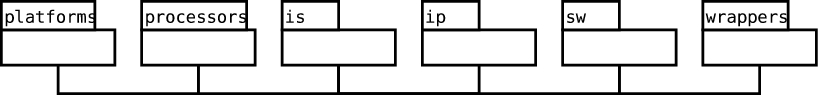
\includegraphics[scale=0.5]{diag_estrutura.png}
\caption{ARP folder structure}
\label{dual:arp}
\end{figure}

This structure will be supported by all examples, so use it. If you
write a wrapper, for example, please put it at the proper dir.
\begin{itemize}
\item \textbf{bin:} ARP scripts
\item \textbf{doc:} Documentation
\item \textbf{platforms:} User and example platforms (including
 top level files and main);
\item \textbf{processors:} ArchC generated simulators used as 
platforms cores;
\item \textbf{is:} Interconnection Structures;
\item \textbf{IP:} IPs, also used as cores;
\item \textbf{sw:} Target software to run on processors;
\item \textbf{wrappers:} All kind of translators between cores, is and 
ips (also between abstraction levels);
\end{itemize}

The naming convention uses a dot to separate versions. If you write a
dual\_mips platform variation, it will be called dual\_mips.XX, where
XX is the version number (however, a name beginning with u\_ to user
defined platforms is desirable to avoid conflict with future
versions). Inside wrappers folder, the dot can be used to specify
different ``languages'' talk by wrapper (ac.simple\_bus\_ua means that
this wrapper talks booth ArchC TLM and simple\_bus\_ua interface).

The static make schema will be ported to GNU autotools soon. Until
that you can use a Makefiles chain to automate compiler tasks.

\subsection{Definition files}

All platforms directories must contain a definition file. It's called defs.arp and contains information about platform structure.

\begin{verbatim}
IP :=
IS := simple_bus_ua
PROCESSOR := mips1-archc2x-branch
SW := fft_shared
WRAPPER := ac.simple_bus_ua
\end{verbatim}

This structure is very similar to makefile structure, but those options can be a list. If the platform use more than one wrapper, for example, the wrapper line will contain a list of space separated wrappers. Blank lists (see IP example above) can be specified too.

\begin{verbatim}
WRAPPER := ac.simple_bus_ua graph_terminal.simple_bus_ua
\end{verbatim}

If you don't plan to use ARP structure you can safely ignore this file.

\subsection{Script}
ARP provides an aiding script. This script is on arp bin folder and is called arp.py. You need Python to run it (tested with version 2.4.2). A symlink at root dir was added in the package for convenience.

This script has three option, passed at command prompt. You can use it by typing the option and the target in any order. The target must be a platform name (the same as the platform directory name) or the keyword \emph{all}, that will do the action over all platforms installed.

\subsubsection{Option --list}
This option list all platforms dependencies. Its useful to see what will be packed.

\begin{verbatim}
$ ./arp --list dual_mips.01
PLATAFORM dual_mips.01 is:
 -- is/simple_bus_ua
 -- processors/mips1-archc2x-branch
 -- sw/fft_shared
 -- wrappers/ac.simple_bus_ua
---
\end{verbatim}

\subsubsection{Option --pack and --unpack}
This option packs platform and all dependencies into a package that can be distributed. It ignores svn directories, but be careful to do a make clean before or your package can be big.

\begin{verbatim}
$ ./arp --pack dual_mips.01
PACK
Packing platform dual_mips.01...
Done.
$ ls -lah dual_mips.01.arp.pack
-rw-r--r-- 1 user users 268K April 14 16:21 dual_mips.01.arp.pack
$ ./arp --unpack dual_mips.01.arp.pack
Unpacking platform dual_mips.01.arp.pack...
Done.
\end{verbatim}

To unpack a package that you downloaded, just execute arp script with unpack option over it. It's safe to discard the package once it is unpacked.

\section{Installing and Running}

Requirements:
\begin{itemize}
\item SystemC 2.1 (tested with v1)
\item TLM library (tested with 1.0)
\item ArchC 2.0 (tested with SVN revision 175)
\item Mips cross-compiler (optional)
\end{itemize}

You can find SystemC and TLM at OSCI \cite{OSCI} site, ArchC and MIPS
cross compiler at ArchC \cite{ARCHC} site. ArchC must be compiled with
TLM enabled (option "with-tlm" passed to configure).

ARP is not a program and all tools are based on interpreted scripts, so you don't need to compile anything. The platforms although must be compiled to run.
To do so, untar ARP, edit Makefile.arp and change the variables to point
your install path correctly:

\begin{verbatim}
SYSTEMC := /home/user/systemc-2.1.v1
ARCHC_PATH := /home/user/archc
TLM_PATH := /home/user/TLM-2005-04-08/tlm
\end{verbatim}

By default, the ``make run'' will take pre compiled binaries from the software folder specified at platform makefile. To compile the binaries, just
execute make at the desired software directory, copy the output to
the correct platform directory and run the simulator manually.

\begin{thebibliography}{99}

\bibitem{ARCHC} ArchC, available at http://www.archc.org
\bibitem{OSCI} SystemC, available at http://www.systemc.org

\end{thebibliography}

\end{document}
